%package list
\documentclass{article}
\usepackage[top=3cm, bottom=3cm, outer=3cm, inner=3cm]{geometry}
\usepackage{graphicx}
\usepackage{url}
\usepackage{hyperref}
\usepackage{array}
%\usepackage{multicol}
\newcolumntype{x}[1]{>{\centering\arraybackslash\hspace{0pt}}p{#1}}
\usepackage[numbers,super]{natbib}
\usepackage{pdfpages}
\usepackage{multirow}
\usepackage{cite}
\usepackage[normalem]{ulem}
% %% Own Packages %%
% \usepackage{csquotes}
% \MakeOuterQuote{"}
\usepackage{listings}



%%%%%%%%%%%%%%%%%%%%%%%%%%%%%%%%%%%%%%%%%%%%%%%%%%%%%%%%%%%%%%%%%%%%%%%%%%%%
%%%%%%%%%%%%%%%%%%%%%%%%%%%%%%%%%%%%%%%%%%%%%%%%%%%%%%%%%%%%%%%%%%%%%%%%%%%%
\newcommand{\csemail}{vmachacaa@ulasalle.edu.pe}
\newcommand{\csdocente}{MSc. Vicente Enrique Machaca Arceda}
\newcommand{\cscurso}{Construcción De Software}
\newcommand{\csuniversidad}{Universidad La Salle}
\newcommand{\csescuela}{Escuela Profesional de Ingeniería de Software}
\newcommand{\cspracnr}{01}
\newcommand{\cstema}{Estándares}
%%%%%%%%%%%%%%%%%%%%%%%%%%%%%%%%%%%%%%%%%%%%%%%%%%%%%%%%%%%%%%%%%%%%%%%%%%%%
%%%%%%%%%%%%%%%%%%%%%%%%%%%%%%%%%%%%%%%%%%%%%%%%%%%%%%%%%%%%%%%%%%%%%%%%%%%%


\usepackage[english,spanish]{babel}
\usepackage[utf8]{inputenc}
\AtBeginDocument{\selectlanguage{spanish}}
\renewcommand{\figurename}{Figura}
\renewcommand{\refname}{Referencias}
\renewcommand{\tablename}{Tabla} %esto no funciona cuando se usa babel
\AtBeginDocument{%
	\renewcommand\tablename{Tabla}
}

\usepackage{fancyhdr}
\pagestyle{fancy}
\fancyhf{}
\setlength{\headheight}{30pt}
\renewcommand{\headrulewidth}{1pt}
\renewcommand{\footrulewidth}{1pt}
\fancyhead[L]{\raisebox{-0.2\height}{
\includegraphics[width=4cm]{../../img/lasalle_black.pdf}}}
\fancyhead[C]{}
\fancyhead[R]{\fontsize{7}{7}\selectfont	\csuniversidad \\ \csescuela \\ \textbf{\cscurso} }
\fancyfoot[L]{MSc. Vicente Machaca}
\fancyfoot[C]{\cscurso}
\fancyfoot[R]{Página \thepage}







\begin{document}

\vspace*{10pt}

\begin{center}
    \fontsize{17}{17} \textbf{ Práctica \cspracnr}
\end{center}
%\centerline{\textbf{\underline{\Large Título: Informe de revisión del estado del arte}}}
%\vspace*{0.5cm}


\begin{table}[h]
    \begin{tabular}{|x{4.7cm}|x{4.8cm}|x{4.8cm}|}
        \hline
        \textbf{DOCENTE} & \textbf{CARRERA} & \textbf{CURSO} \\
        \hline
        \csdocente       & \csescuela       & \cscurso       \\
        \hline
    \end{tabular}
\end{table}


\begin{table}[h]
    \begin{tabular}{|x{4.7cm}|x{4.8cm}|x{4.8cm}|}
        \hline
        \textbf{PRÁCTICA} & \textbf{TEMA} & \textbf{DURACIÓN} \\
        \hline
        \cspracnr         & \cstema       & 3 horas           \\
        \hline
    \end{tabular}
\end{table}


\section{Datos de los estudiantes}
\begin{itemize}
    \item Grupo: 1
    \item Integrantes:
          \begin{itemize}
              \item Elvis Andre Cruces Gomez
              \item Yoshiro Milton Miranda Valdivia
              \item José Alfredo Pinto Villamar
          \end{itemize}
\end{itemize}





\section{NTP-ISO/IEC 12207:2016}\label{sec:Intro}
\subsection{Introducción}

\begin{enumerate}
    \item \textbf{Motivación:}

    La \nocite{ISO12207} NTP ISO/IEC 12207 nació en base a la norma seguida en noviembre de
    2002, la ISO/IEC 15288, la cual abarca el tema de los procesos del ciclo de
    vida del sistema. En nuestra norma se buscaba que el software y sus procesos
    de diseño se consideren como una parte integral del sistema y de sus propios
    procesos y que no los trataran de manera separada.

    La creación de esta norma se realizo para poder ayudar a las
    organizaciones a establecer entornos de los procesos deseados por la empresa,
    así como también, para evaluar ciertos criterios que apoyen la mejora del
    proceso organizacional. Además, también puede ser utilizado en proyectos
    para ayudar a seleccionar, estructurar y emplear elementos de un conjunto
    establecidos de procesos del ciclo de vida y así proporcionar productos y
    servicios.

    Esta norma se puede aplicar en la adquisición de productos y servicios
    de sistemas y software, al desarrollo, operación, mantenimiento y
    disposición de los productos de software y del software en general,
    independientemente de si se ejecute de manera interna o externa de una
    organización.

    \item \textbf{Objetivo del estándar:}
    
    El objetivo de esta norma es proporcionar un conjunto definido de
    procesos para facilitar la comunicación entre aquellos que adquieren los
    productos que vienen a ser los clientes, usuarios u organizaciones, los
    proveedores que son aquellos que ofrecen el producto o vendedores y
    aquellos interesados en el ciclo de vida de un producto de software.

    Sobre todo, la norma fue diseñada para utilizarla por dos partes, ya
    sean organizaciones diferentes o que ambas partes pertenezcan a la misma
    organización, esto dependiendo de si existe o no un acuerdo informal o un
    contrato legalmente vinculante. Cabe resaltar que la norma se utiliza a
    través de un conjunto de procesos autoimpuestos, el cual no impide el uso de
    la norma por parte de los proveedores o de los desarrolladores de software.

\end{enumerate}

\subsection{Historia y Versiones del Estandar}\label{sec:Historia}

La primera versión de la ISO/IEC 12207 fue publicada en 1995. Los
desarrolladores de dicho estándar vieron la necesidad de describir los procesos,
las actividades y las tareas de tales procesos con el fin de facilitar el
desarrollo del software en situaciones que involucran a dos partes. Sin embargo,
la ISO/IEC 12207:1995 está orientada hacia qué necesidades se deben satisfacer.
Describe los procesos en términos de actividades y tareas. En el mismo marco
temporal, la industria del software se dio cuenta que tenía la misma importancia,
la necesidad de evaluar la capacidad del proceso en una escala continua de una
manera comparable y repetible para dar soporte a la mejora del proceso y a la
reducción del riesgo durante la selección del proveedor.

La determinación de la capacidad de procesos requiere que sus descripciones incluyan una declaración
clara del propósito del proceso y una descripción de los resultados esperados.
Estas declaraciones de propósito y resultados fueron omitidas en la ISO/IEC
12207:1995 y fueron proporcionadas por las enmiendas de dicho estándar en los
años 2002 y 2004. Tales enmiendas también añadieron un número de procesos de
nivel detallado para facilitar la evaluación correcta de los procesos del ciclo
de vida del software completo.

Aunque la ISO/IEC 12207 trató a los procesos del ciclo de vida del software dentro de un contexto de sistemas, fue evidente que
se necesitaba un estándar similar en el dominio de los sistemas. La ISO/IEC
15288 , publicada en noviembre de 2002, cubrió esa necesidad. Los
desarrolladores de este estándar se beneficiaron de la experiencia ganada en el
desarrollo de la enmienda de la ISO/IEC 12207 y comprendieron las necesidades
tal como se expresan en la ISO/IEC 15504; por lo tanto, los procesos en la norma
ISO/IEC 15288 se expresan en términos de propósitos y resultados con la
descripción de las actividades requeridas para lograr tales resultados.

El desarrollo escalonado de las enmiendas de la ISO/IEC 12207 con la ISO/IEC 15288
y un enfoque inicial diferente de la ISO/IEC 12207 ocasionó algunas dificultades
en la aplicación de la enmienda de la ISO/IEC 12207, así como en la aplicación
de los estándares del ciclo de vida del sistema y del software juntos. Un
proyecto de armonización dentro de la ISO/IEC JTC 1/SC 7 una revisión paralela,
cuidadosamente controlada de la ISO/IEC 12207 e ISO/IEC 15288, y el desarrollo
del informe técnico ISO/IEC 24748, el cual proporciona directrices para ambas
normas es el primer y gran paso hacia un conjunto integrado de normas que
describen los ciclos de vida del software y del sistema.

\subsection{Caracteristicas del Estandar}\label{sec:Caracteristicas}
\subsubsection{Características Principales}
    \begin{figure}[!h]
        \centering
        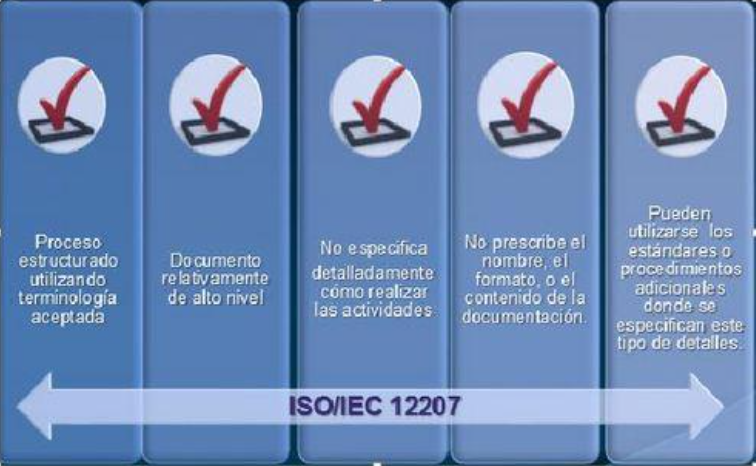
\includegraphics[scale=.37]{caracteristicas1.png}
        \caption{Las caractiristicas principales del ISO/IEC 12207:2016}
    \end{figure}
\subsubsection{Procesos}
La estructura general que compone a esta normativa es la siguiente y se
clasifican en tres tipos de procesos:
\begin{enumerate}
    \item \textbf{Procesos Primarios}
            \begin{enumerate}
                \item \textbf{Adquisición: }Identificar la
                necesidad, preparar una solicitud y seleccionar un proveedor.

                \item \textbf{Suministro: }Determinar
                procedimientos y recursos para gestionar el proyecto.

                \item \textbf{Desarrollo: }Contiene las
                actividades del desarrollo y una estructura definida para el
                desarrollador o para la empresa desarrolladora.

                \item \textbf{Mantenimiento: }Modificar el
                producto de software preservando su integridad. Incluye la
                migración y retirada del producto.

                \item \textbf{Operación: }Cubre la operación del
                producto de software y apoyo a los usuarios. Las actividades y
                tareas hacen referencia al sistema.
            \end{enumerate}

    \item \textbf{Procesos de Soporte}
    \begin{enumerate}
        \item \textbf{Documentación: }El propósito de este es obtener y
        persistir información.

        \item \textbf{Administración de la configuración: }El propósito
        de este proceso es identificar, definir y versionar, mediante líneas
        bases, los elementos del sistema, así como también asegurar la
        completitud y correctitud de los elementos que pertenecen a la
        configuración, de controlar su manejo, persistencia y entrega de los
        mismos.

        \item \textbf{Aseguramiento de calidad: }El propósito de este
        proceso es proveer de mecanismos, para objetiva e independientemente
        asegurar que los productos y/o servicios cumplan con los estándares y
        requerimientos establecidos.

        \item \textbf{Verificación: }El propósito de este proceso es
        proveer las evaluaciones referentes a la verificación de un producto o
        servicio de una actividad dada.

        \item \textbf{Validación: }El propósito de este proceso es
        determinar si un sistema ya construido cumple con las especificaciones y
        requerimientos para los cuales fue realizado.

        \item \textbf{Revisiones conjuntas: }El propósito de este
        proceso es proveer un marco que favorezca la integración entre inspector
        e inspeccionado.

        \item \textbf{Resolución de problemas: }El propósito de este
        proceso es proveer mecanismos para la creación de procesos capaces de
        resolver problemas y tomar acciones correctivas para remover nuevos
        problemas detectados.
    \end{enumerate}
    \item \textbf{Procesos Organizacionales}
        \begin{enumerate}
            \item \textbf{Administración: }El propósito de este
            proceso es proveer actividades y tareas genéricas que pueden
            emplearse y ajustarse para gestionar otros procesos.

            \item \textbf{Infraestructura: }El propósito de este
            proceso es definir las actividades necesarias para establecer y
            mantener la infraestructura (hardware, software, estándar,
            herramientas, etc.) necesaria por otros procesos.

            \item \textbf{Mejoras: }El propósito de este proceso es
            proveer de actividades básicas y de alto nivel para establecer,
            evaluar, medir, controlar y mejorar un proceso de ciclo de vida del
            software.

            \item \textbf{Entrenamiento: }El propósito de este
            proceso es proporcionar y mantener al personal capacitado.

            \begin{figure}[pbth]
                \centering
                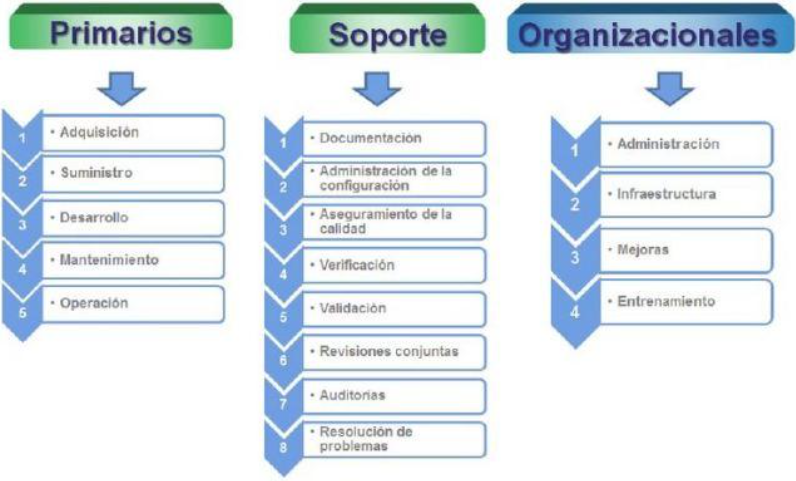
\includegraphics[scale=.37]{caracteristicas2.png}
                \caption{Procesos Primarios del ISO/IEC 12207:2016}
            \end{figure}

        \end{enumerate}

\subsubsection{Factores para aplicar al estándar}

        \begin{enumerate}
            \item \textbf{Ciclo de vida del sistema}\\
                En general un ciclo de vida, cubre las fases de
                requisitos, análisis, diseño, documentación y pruebas.

            \item \textbf{Tipo de software}\\
                El tipo del software del proyecto debe ser
                determinado como nuevo software, firmware, reutilización de uno
                existente, software indebido, software independiente, etc.
            
            \item \textbf{Rol en el ciclo de vida}\\
                El usuario dentro del estándar, se debe
                determinar si es un comprador, un proveedor, un desarrollador,
                un operador o el de soporte.

            \item \textbf{Modelo de desarrollo}\\
                En general un ciclo de vida, cubre las fases de
                requisitos, análisis, diseño, documentación y pruebas.
            
            \item \textbf{Características del proyecto}\\
                Los requerimientos y especificaciones del
                producto o servicio, dominan la determinación y selección de
                procesos, actividades y tareas.

            \item \textbf{Documentación}\\
                El estándar ISO/IEC 12207 proporciona resultados
                de las tareas y actividades. Se va a determinar qué resultados
                son necesarios, como deben de ser combinados, empaquetados y
                distribuidos.
            
            \item \textbf{Cláusulas de la norma}\\
                Se deben controlar las cláusulas relacionadas
                con la ingeniería, en la que el usuario debe de actuar con
                precaución y juicio técnico, influyendo en la documentación.
            
        \end{enumerate}
        
\end{enumerate}

\subsection{Caso de estudio}\label{sec:Caso de Estudio}

Para este caso de estudio, hemos escogido una tesis \nocite{quinteros_estefani2019} que habla
sobre el proceso de adquisición de software como servicio o producto para
OSIPTEL. La cual propone la una metodología integrada de gestión basada en la
gestión por proceso y la NTP 12207:2016. La metodología integrada de gestión
(MIG) presenta dos pilares fundamentales. Siendo el primero un modelo basado en
tres niveles: Estratégico, Táctico y Operativo, los cuales guardan una relación
estrecha con la estructura de OSIPTEL. Y el segundo modelo de capacidad de
procesos. El modelo de gestión guarda absoluta relación con los procesos de
software basado en la NTP 12207:2016.

\begin{figure}[!h]
    \centering
    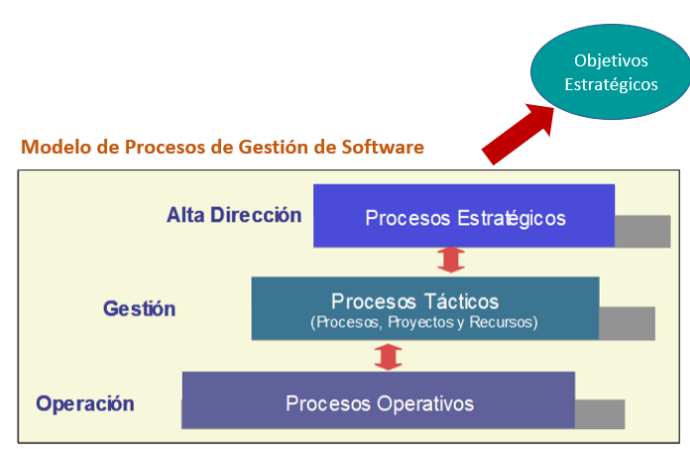
\includegraphics[scale=.37]{caso1.png}
    \caption{Modelo de Procesos de Gestión de Software}
\end{figure}

Así mismo, el modelo de capacidad de procesos establece la madurez de cada
proceso que se implemente. Este siguiente modelo presenta 5 niveles:

\begin{figure}[!h]
    \centering
    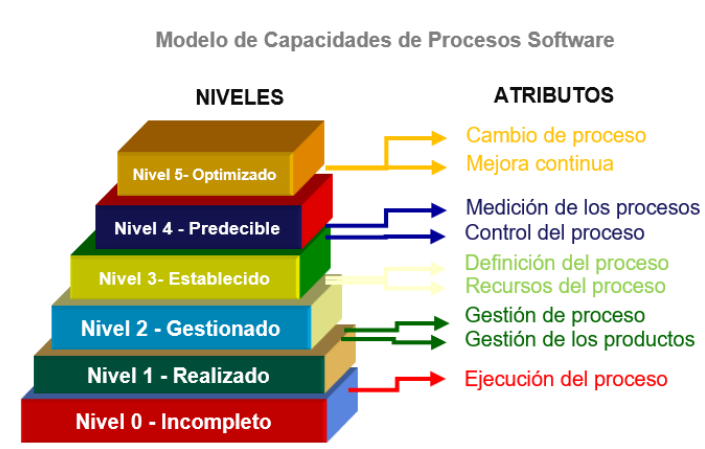
\includegraphics[scale=.37]{caso2.png}
    \caption{Modelo de Procesos de Gestión de Software}
\end{figure}

Y finalmente hablan de la identificación y mejora de los formatos de metodología
integrada de gestión (MIG) y hacen una tabla siguiendo los lineamientos de la
NTP ISO/IEC 12207:2016.


\begin{table}[h]
    \begin{tabular}{|l|l|l|}
    \hline
    \multicolumn{1}{|c|}{\textbf{AREA}} & \multicolumn{1}{c|}{\textbf{SUB AREA}} & \multicolumn{1}{c|}{\textbf{DOCUMENTO}}     \\ \hline
    Gestión Estratégico                 & Gestión Estratégico                    & Plan estratégico de TI                      \\ \hline
    Gestión Estratégico                 & Gestión Estratégico                    & Acta de Reunión de Comité de Sistemas       \\ \hline
    Gestión Estratégico                 & Gestión Estratégico                    & Comunicado Comité Comité de Sistemas        \\ \hline
    Gestión Táctica                     & Gestión de Proyectos                   & Solicitud de Usuario                        \\ \hline
    Gestión Táctica                     & Gestión de Proyectos                   & Ficha del Proyecto                          \\ \hline
    Gestión Táctica                     & Gestión de Proyectos                   & Informe de Viabilidad                       \\ \hline
    Gestión Táctica                     & Gestión de Proyectos                   & Términos de Referencia                      \\ \hline
    Gestión Táctica                     & Gestión de Proyectos                   & Definición Inicial de Requerimientos        \\ \hline
    Gestión Táctica                     & Gestión de Proyectos                   & Bases Administrativas                       \\ \hline
    Gestión Táctica                     & Gestión de Proyectos                   & Propuesta de Solución                       \\ \hline
    Gestión Táctica                     & Gestión de Proyectos                   & Plan General del Proyecto                   \\ \hline
    Gestión Táctica                     & Gestión de Proyectos                   & Plan de Gestión de Desarrollo               \\ \hline
    Gestión Táctica                     & Gestión de Proyectos                   & Plan de Gestión de la Migración             \\ \hline
    Gestión Táctica                     & Gestión de Proyectos                   & Plan de Gestión de la Calidad               \\ \hline
    Gestión de Proyectos                & Gestión de Proyectos                   & Plan de Gestión de Entrenamiento al Usuario \\ \hline
    \end{tabular}
\end{table}

\pagebreak
\subsection{Conclusiones}\label{sec:conclusiones}
En conclusión, la norma NTP ISO/IEC 12207 tiene la función de ayudar a
organizaciones y empresas a que exista una mejor comunicación entre los
stakeholder para así tener mejores ventas, es decir, el ofrecimiento de sus
productos o servicios.

%\clearpage
%\bibliographystyle{apalike}
\bibliographystyle{IEEEtranN}
\nocite{*}
\bibliography{refs.bib}
%\bibliography{bibliography}

\section{Repositorio}\label{sec:Repositorio}
\begin{itemize}
    \item {\color{blue}\href{https://github.com/pintovillamar/software-construction/tree/main/pract01/NTPISOIEC12207_2016}{Practica 1}}
\end{itemize}


\end{document}